\documentclass[10pt,a4paper]{article}
\usepackage[utf8]{inputenc}
\usepackage[english]{babel}
\usepackage{amsmath}
\usepackage{amsfonts}
\usepackage{amssymb}
\usepackage{graphicx}
\usepackage{hyperref}
\usepackage{listings}

\graphicspath{ {../images/} }

\author{\href{https://github.com/ManuelPrandini}{Manuel Prandini}, \href{https://github.com/dsforza96}{Davide Sforza}, \href{https://github.com/giovannivarr}{Giovanni Varricchione}}
\title{Generating Trees with a Space Colonization Algorithm}

\begin{document}
\maketitle

A parallel C++ tool to procedurally generate trees using a space colonization
algorithm. \\

The project is based on the \href{https://github.com/xelatihy/yocto-gl}{Yocto/GL} and the \href{http://math.lbl.gov/voro++/}{Voro++} libraries. The algorithm used is taken from the paper "Modeling Trees with a Space Colonization Algorithm" by Runions, Lane and Prusinkiewicz; while the method to evaluate the parallel transport frame is taken from "Parallel Transport Approach to Curve Framing" by Hanson and Ma. \\

The texture we have used to generate the models are all taken from the website \href{https://textures.com}{textures.com}.

\section{Implementation}

The basic input for the tool is the shape of the tree's crown and a number ofattraction points, which will be randomly placed in the crown. After this, the growth begins and the tool uses the \textbf{Voro++} library to compute two Voronoi Diagrams, one for the attraction points and the other for the tree nodes. We then loop on the nodes (for each one we create a new thread), we search for the closest attraction point  within a certain distance called \textit{radius of influence} for each tree node (we use the attraction points' loop to search for this) and compute the \textit{growth} by adding a new node which will be closer to the attraction point. Once a tree node is within the \textit{kill distance} of an attraction point, the point is considered dead and will not influence the growth in future iterations.

The growth loop continues as long as:
 \begin{itemize}
 	\item there is at least one attraction point which is \textbf{not} dead
  	\item the max number of iterations (which is an optional input parameter) has not been reached yet
  \end{itemize}

Once the growth has ended, the model is created; in order to create this, we associate each node to a certain radius (for leaves, i.e. the nodes which are childless, we use a constant value) which is calculated as the e-th root of the sum of the children's radius elevated to the e  (where e = 2.05): the radius is then used to create the cylinder which connects the node to its father. \\
The cylinder's direction is based off of the father's parallel transport frame.

\section{Parameters}

The following parameters can be used as inputs:
\begin{itemize}
	\item \texttt{-N int} to specify the number of attraction points to be randomly placed
	\item \texttt{-D float} to specify the distance between a \textit{father} node and one of its \textit{children} nodes
	\item \texttt{-di float} to specify the radius of influence
	\item \texttt{-dk float} to specify the kill distance
	\item \texttt{-i int} to specify the max number of iterations
	\item \texttt{-l path} d to specify the leaves/flowers texture to use in the generation
	\item \texttt{-o path} to specify the output directory
	\item the crown shape can be chosen from the following options:
    	\begin{itemize}
    		\item \texttt{CONE float}: specifying the crown's height
    		\item \texttt{DOME float}: specifying the crown's radius
    		\item \texttt{CYLINDER float float}: specifying the crown's height and the radius
    		\item \texttt{BEZIER float float float float float float float float}: specifying the four points which define the spline
    	\end{itemize}
	\item the trunk's height, i.e. the distance between the root and the crown
\end{itemize}

It is possible to display an help message using the \texttt{-h} parameter.

\section{Examples}

\subsection{Simple Tree}

\begin{centering}
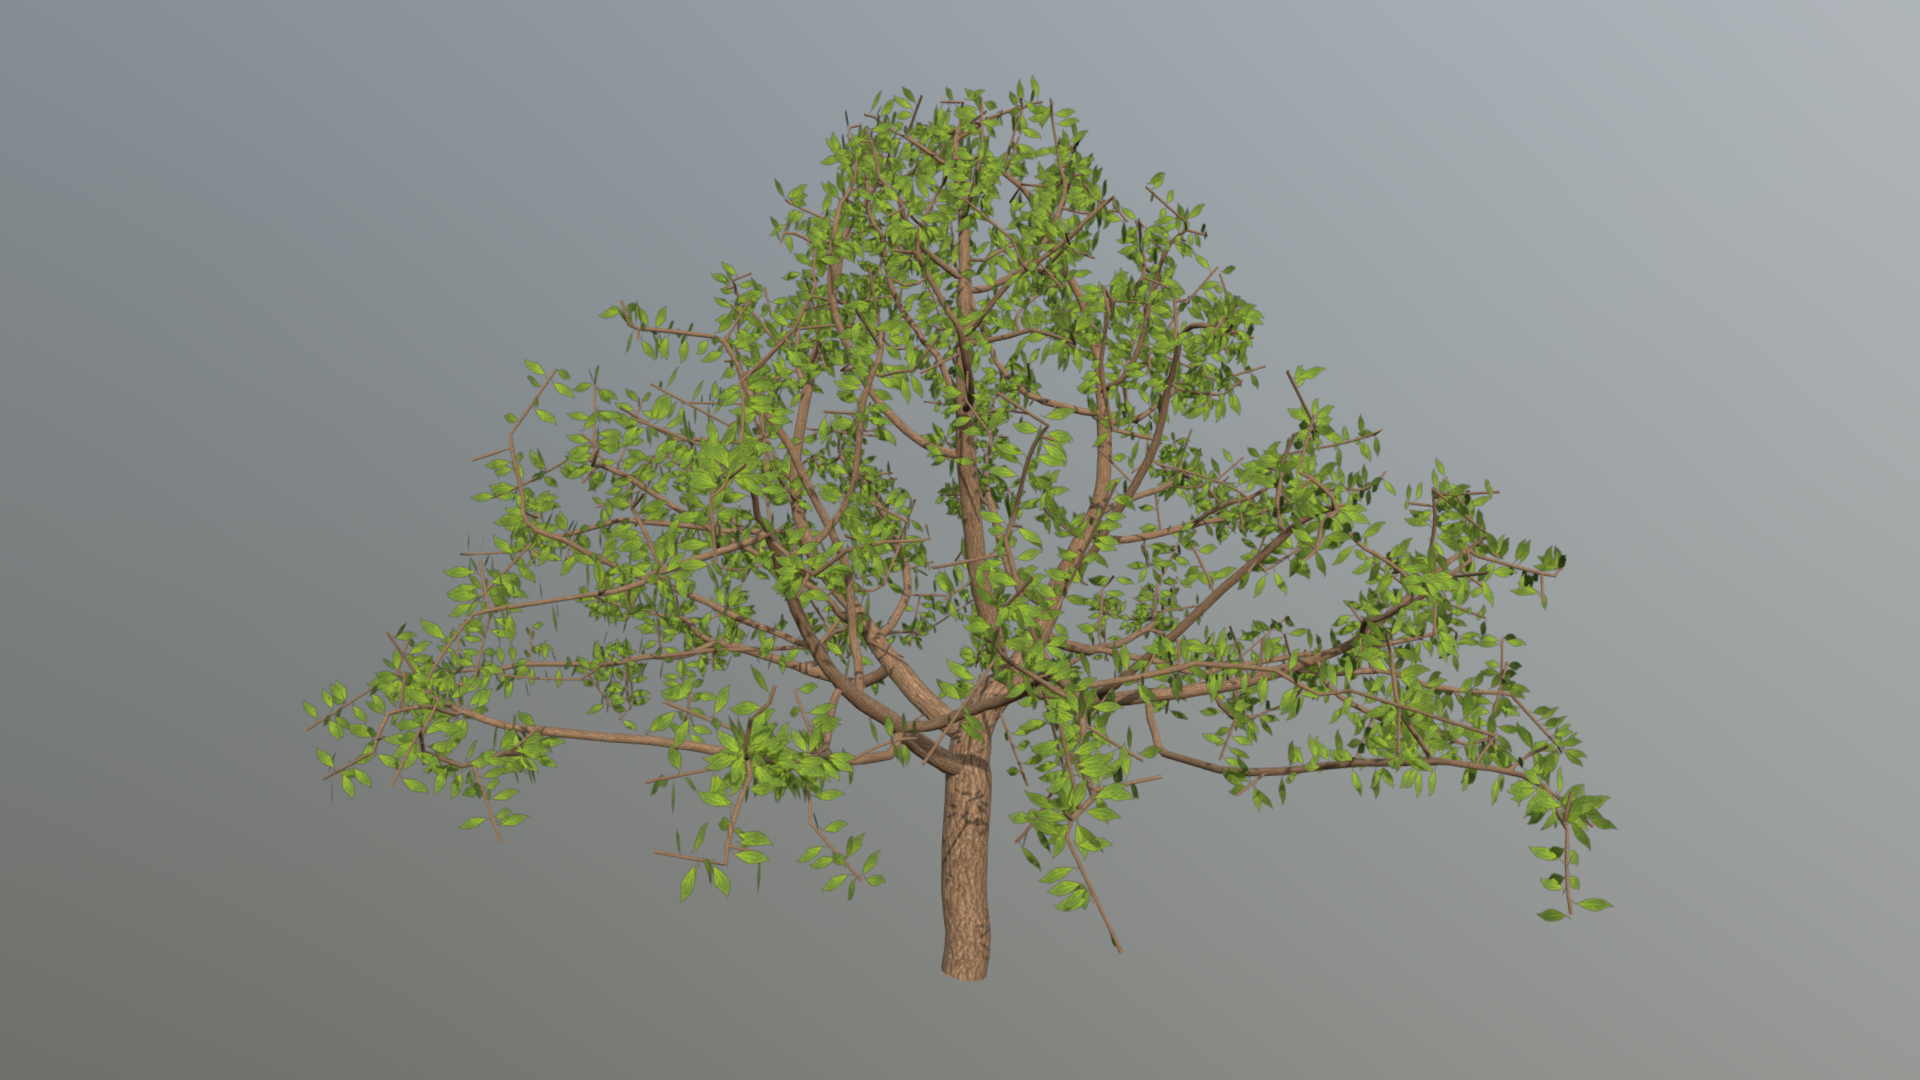
\includegraphics[scale=.2]{simple.png}
\end{centering}

\begin{centering}
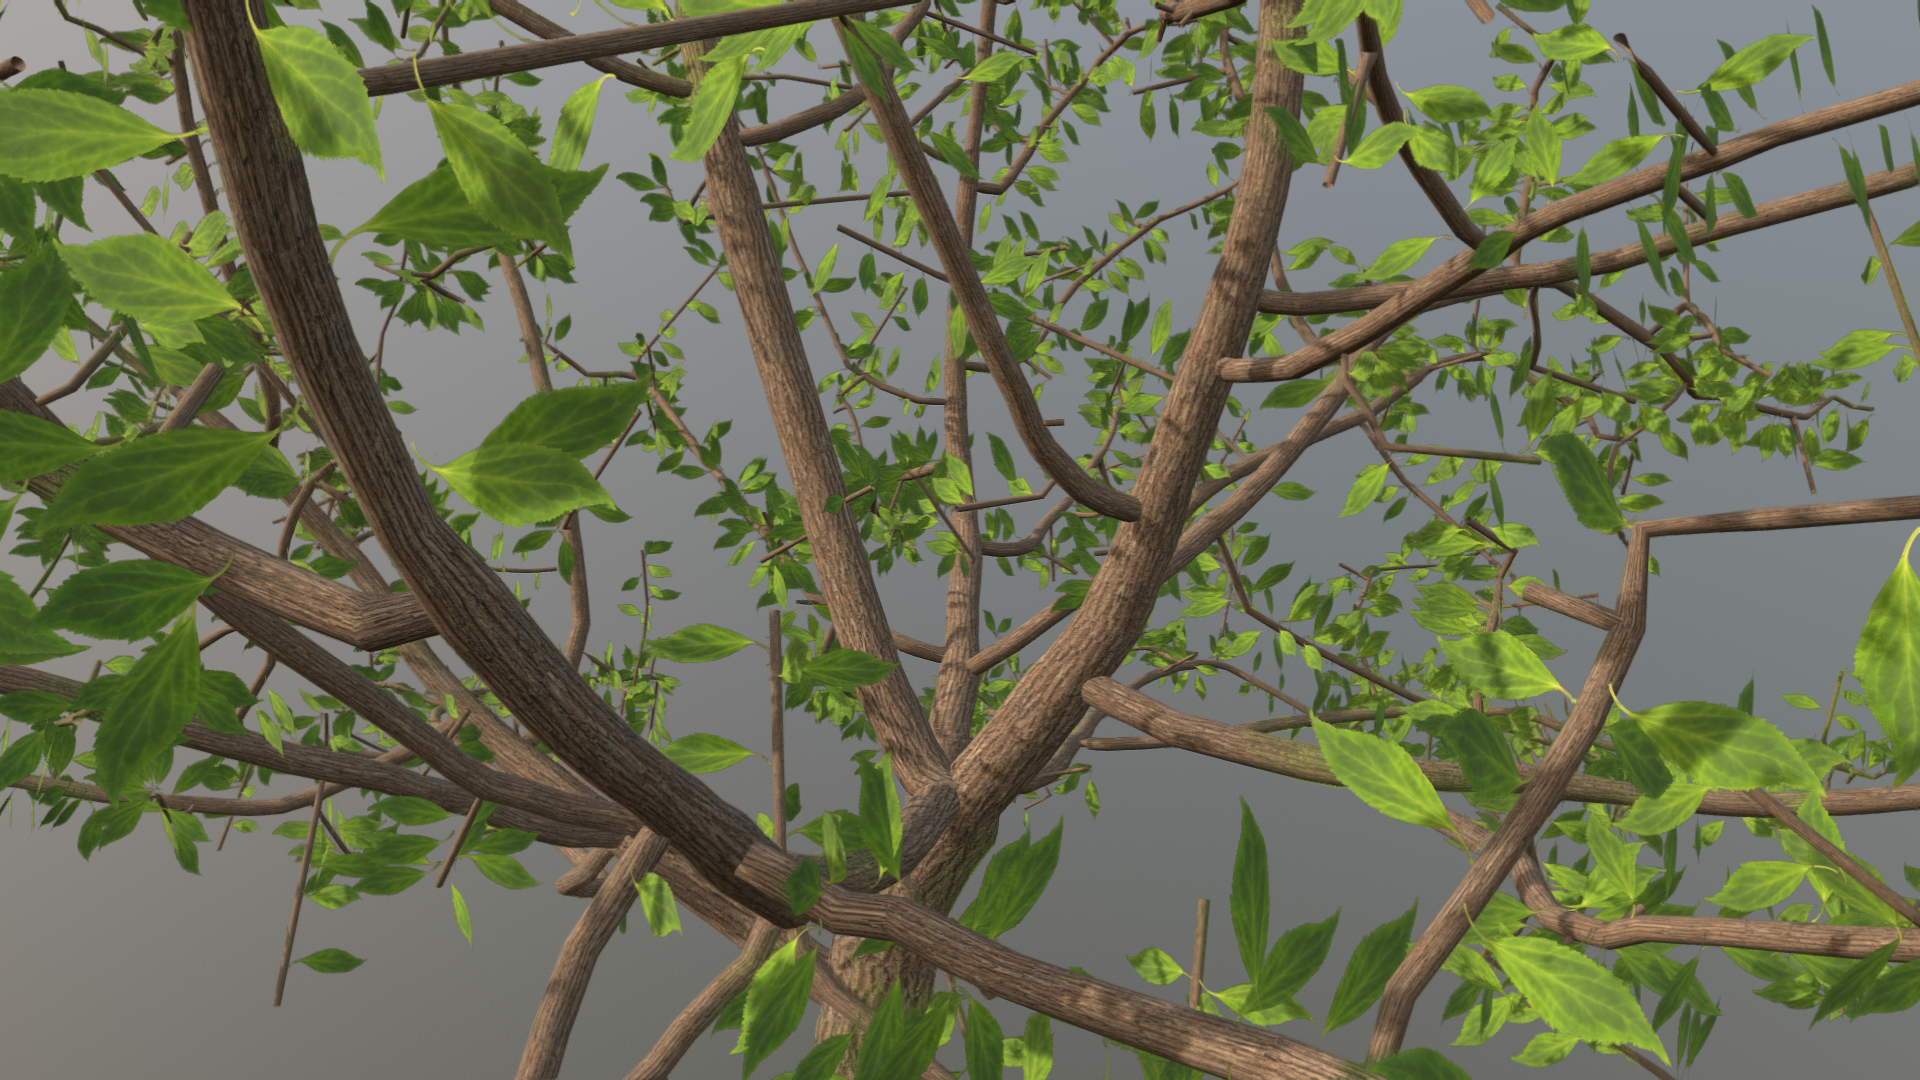
\includegraphics[scale=.2]{simple_detail.png}
\end{centering}

\texttt{bin/tree-gen -N 800 DOME 2 6}

\subsection{Fir}

\begin{centering}
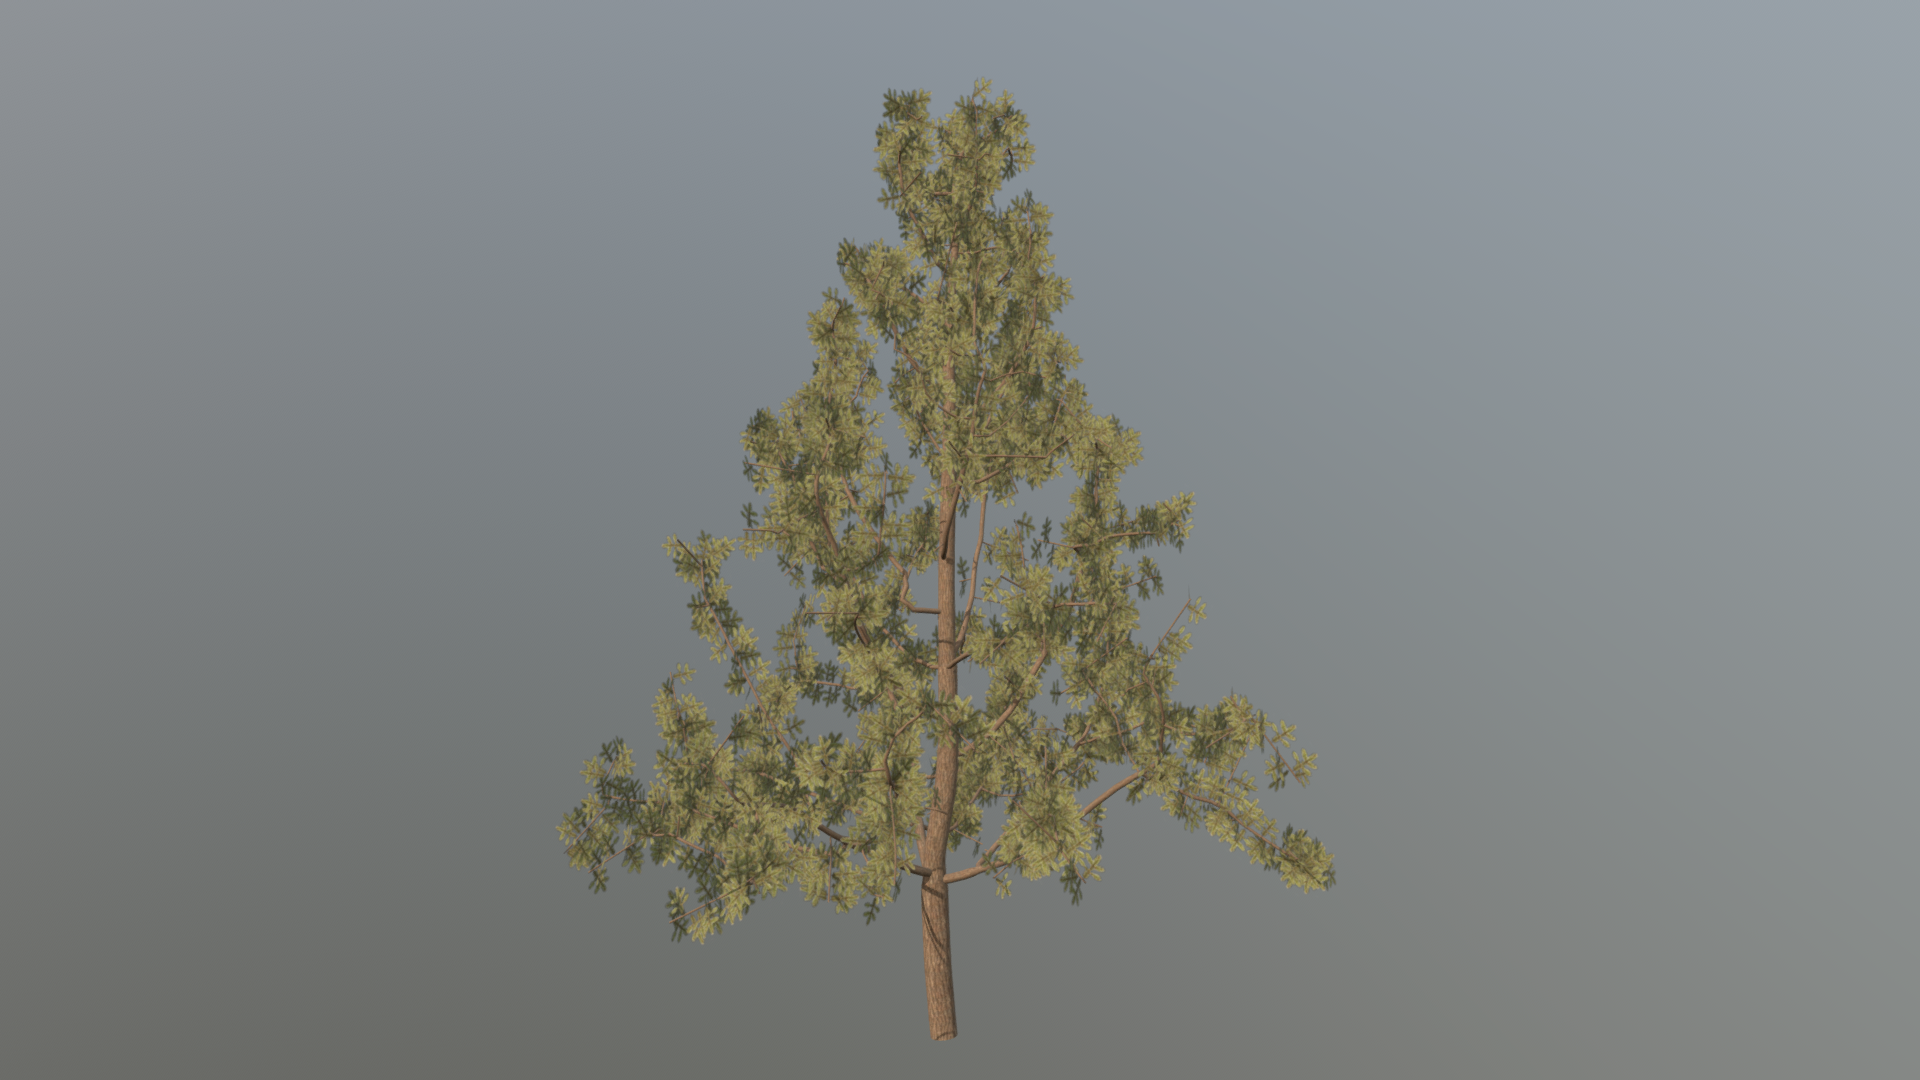
\includegraphics[scale=.2]{fir.png}
\end{centering}

\texttt{bin/tree-gen -di 50 -l resources/needle\_leaf.png CONE 2 10 5}

\subsection{Cypress}

\begin{centering}
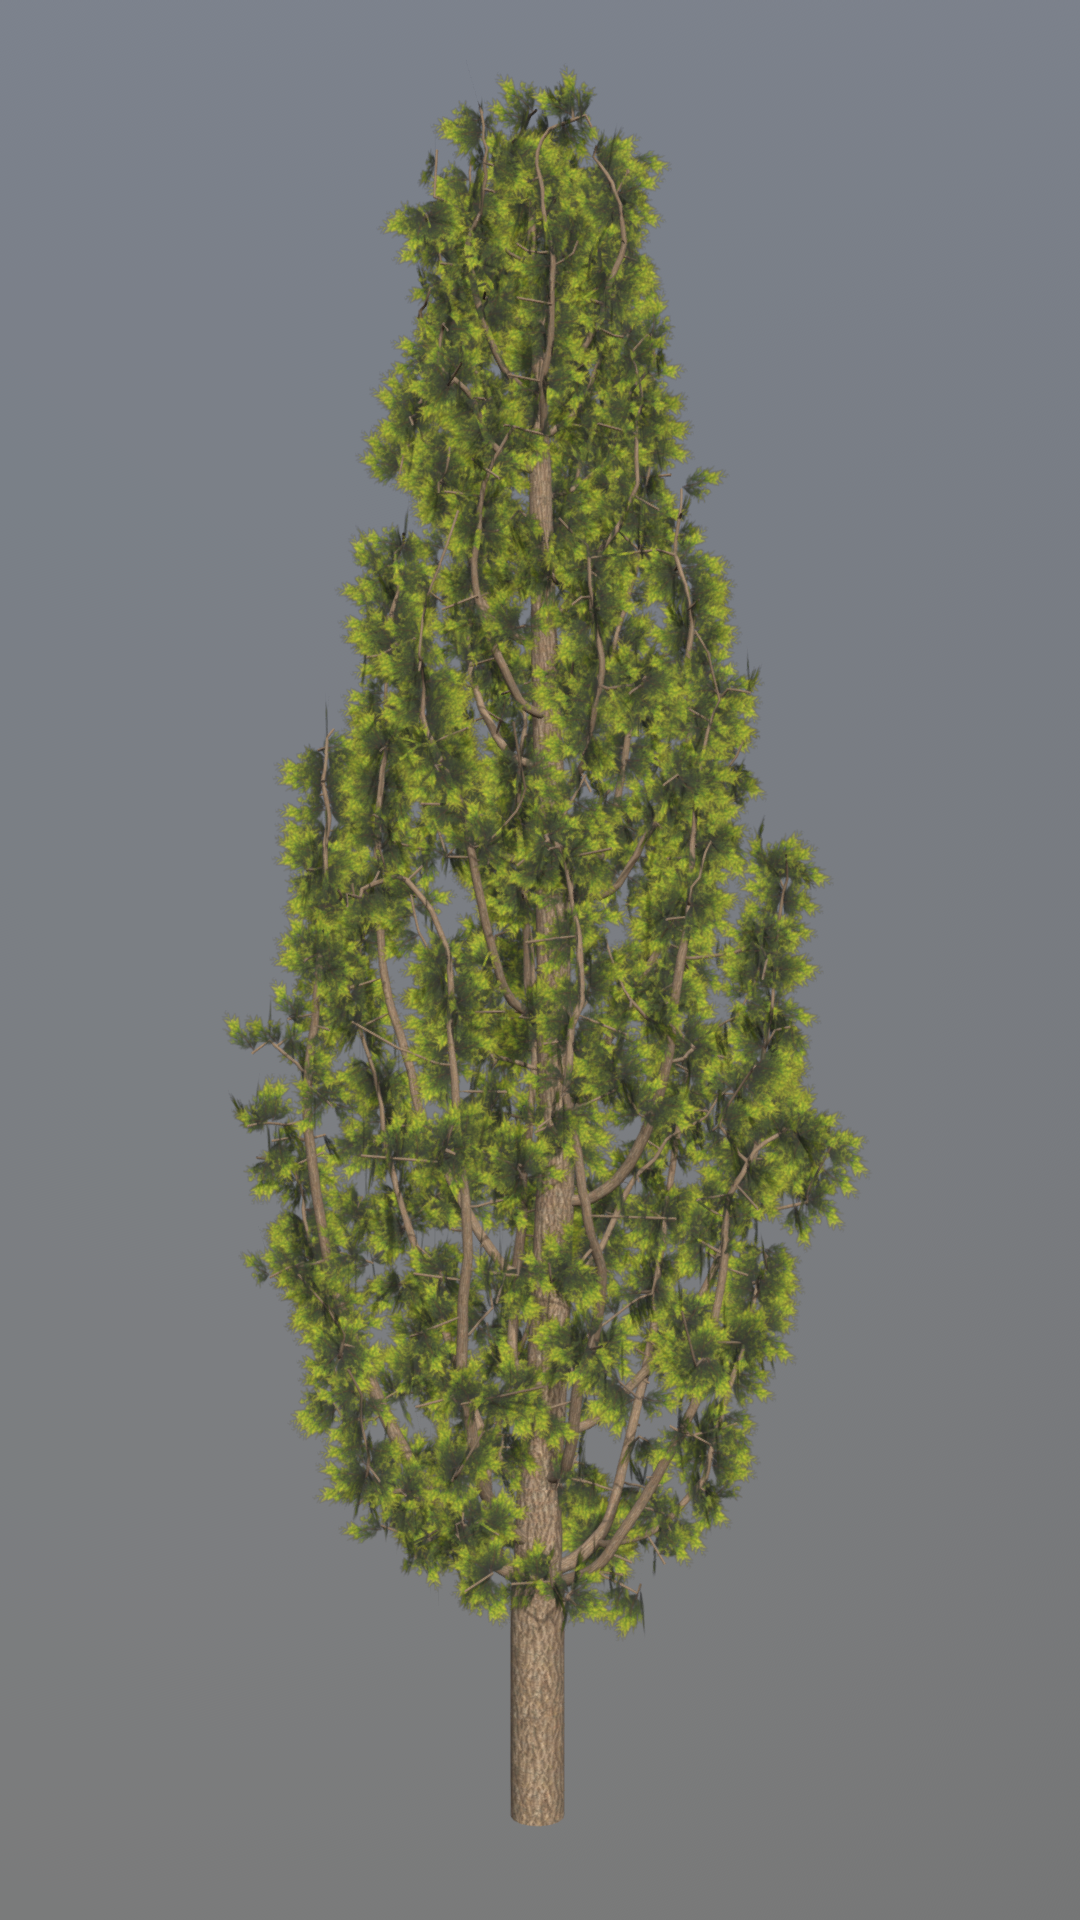
\includegraphics[scale=.28]{cypress.png}
\end{centering}

\texttt{bin/tree-gen -N 1000 -di 50 -l resources/small\_branch.png BEZIER 2 0 1 2 4.5 7 0.5 12 1}

\end{document}